
\begin{enumerate}[label=\thesection.\arabic*,ref=\thesection.\theenumi]
\numberwithin{equation}{enumi}
\numberwithin{figure}{enumi}
\numberwithin{table}{enumi}
\item 
\label{chapters/12/8/1/1}
	\begin{figure}[!h]
		\centering
 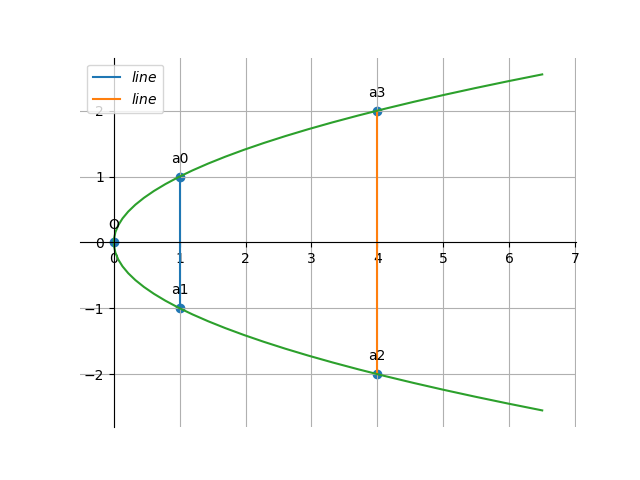
\includegraphics[width=\columnwidth]{chapters/12/8/1/1/figs/conics1.png}
		\caption{}
		\label{fig:12/8/1/1}
  	\end{figure}

The parameters of the conic are
\begin{align}
	\vec{V} = \myvec{0 & 0\\0 & 1},
	\vec{u} = -\frac{1}{2}\myvec{ 1\\0},
	f = 0
	%\\
\end{align}
\iffalse
The point of intersection of the lines $x=1$ and $x=4$ to the parabola is given by


The points of intersection of the line 
\begin{align}
	L: \quad \vec{x} = \vec{q} + \kappa \vec{m} \quad \kappa \in \mathbf{R}
\label{eq:conic_tangent}
\end{align}
with the conic section are given by
\begin{align}
\vec{x}_i = \vec{q} + \kappa_i \vec{m}
\label{eq:conic_tangent_pts}
\end{align}
%
where
{\tiny
\begin{multline}
\kappa_i = \frac{1}
{
\vec{m}^T\vec{V}\vec{m}
}
\lbrak{-\vec{m}^T\brak{\vec{V}\vec{q}+\vec{u}}}
\\
\pm
\rbrak{\sqrt{
\sbrak{
\vec{m}^T\brak{\vec{V}\vec{q}+\vec{u}}
}^2
-
\brak
{
\vec{q}^T\vec{V}\vec{q} + 2\vec{u}^T\vec{q} +f
}
\brak{\vec{m}^T\vec{V}\vec{m}}
}
}
\label{eq:tangent_roots}
\end{multline}
}
\fi
For the line $x-1=0$, the parameters are  
\begin{align}
	\vec{q}_2=\myvec{1\\0},
	\vec{m}_2=\myvec{0\\1}
\end{align}
Substituting from the above in 
\eqref{eq:tangent_roots},
\begin{align}
\kappa_i=1,-1
\end{align}
yilelding 
the points of intersection 
\begin{align}
	\vec{a}_0=\myvec{1\\1},
	\vec{a}_1=\myvec{1\\-1}
\end{align}
Similarly, 
for the line $x-4=0$ 
\begin{align}
\vec{q_1}=\myvec{4\\0},
\vec{m_1}=\myvec{0\\1}
\end{align}
yielding
\begin{align}
\kappa_i=2,-2
\end{align}
from which, the points of 
intersection are
\begin{align}
\vec{a_3}=\myvec{4\\2},
\vec{a_2}=\myvec{4\\-2}
\end{align}
		See \figref{fig:12/8/1/1}.
Thus, 
the area of the parabola in between the lines $x=1$ and $x=4$ is given by
\begin{align}
\int_{0}^{4} \ \sqrt{x} \,dx-\int_{0}^{1} \ \sqrt{x} \,dx
=14/3
\end{align}

\item 
\label{chapters/12/8/1/2}
	\begin{figure}[H]
		\centering
 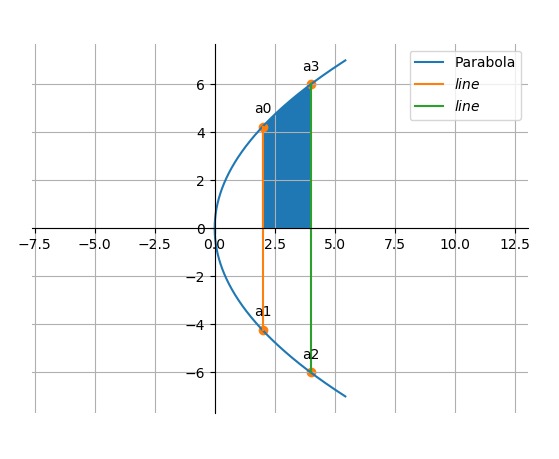
\includegraphics[width=0.75\columnwidth]{chapters/12/8/1/2/figs/conics1.png}
		\caption{}
		\label{fig:12/8/1/2}
  	\end{figure}
The parameters of the conic are
\begin{align}
 \vec{V} = \myvec{0 & 0\\0 & 1},
	\vec{u} = \frac{9}{2}\myvec{1 \\0},
 f = 0.
\end{align}
The parameters of 
the line $x-2=0$ are
\begin{align}
\vec{q_2}=\myvec{2\\0},
\vec{m_2}=\myvec{0\\1}
\end{align}
Substituting in 
\eqref{eq:tangent_roots},
\begin{align}
\kappa_i=\pm 3\sqrt{2}
\end{align}
yielding
\begin{align}
\vec{a_0}=\myvec{2\\3\sqrt{2}},
\vec{a_1}=\myvec{2\\-3\sqrt{2}}.
\end{align}
Similarly, 
for the line $x-4=0$,
\begin{align}
\vec{q_1}=\myvec{4\\0},
\vec{m_1}=\myvec{0\\1}
\end{align}
yielding
\begin{align}
\kappa_i=\pm 6.
\end{align}
Thus, 
\begin{align}
\vec{a_3}=\myvec{4\\6},
\vec{a_2}=\myvec{4\\-6}
\end{align}
and 
		from \figref{fig:12/8/1/2},
the 
desired area of the parabola is
\begin{align}
\int_{0}^{4} \ 3\sqrt{x} \,dx-\int_{0}^{2} \ 3\sqrt{x} \,dx
=16-4\sqrt{2}
\end{align}

\item Find the area of the region bounded by ${x}^2
= 4{y}$, ${y} = 2$, ${y} = 4$ and the y-axis in the
first quadrant.
\label{chapters/12/8/1/3}
\item Find the area of the region bounded by the ellipse \(\frac{{x}^2}{16}\ + \frac{{y}^2}{9} = 1\)
\label{chapters/12/8/1/4}
\item Find the area of the region bounded by the ellipse \(\frac{{x}^2}{4}\ + \frac{{y}^2}{9} = 1\)
\label{chapters/12/8/1/5}
%\item 
%\label{chapters/12/8/1/3}
%%	\begin{figure}[H]
		\centering
 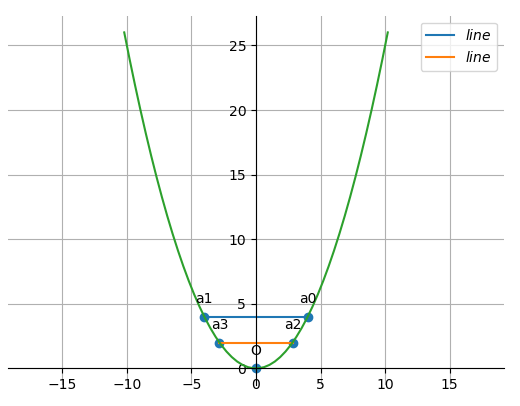
\includegraphics[width=0.75\columnwidth]{chapters/12/8/3/3/figs/conic.png}
		\caption{}
		\label{fig:12/8/3/3}
  	\end{figure}
The conic parameters are
\begin{align}
	\vec{V} = \myvec{1 & 0\\0 & 0},
	\vec{u} = \myvec{0\\-2},
	f = 0
	%\\
\end{align}
The vector parameters of 
$y-4=0$
are
\begin{align}
	\vec{h}_1=\myvec{0\\4},
	\vec{m}_1=\myvec{1\\0}
\end{align}
Substituting the above in \eqref{eq:tangent_roots},
\begin{align}
\kappa_i=4,-4
\end{align}
yielding
the points of intersection with the parabola as
\begin{align}
\vec{a}_0=\myvec{4\\4},
\vec{a}_1=\myvec{-4\\4}
\end{align}
Similarly, for 
the line $y-2=0$, the vector parameters are
\begin{align}
\vec{h}_2=\myvec{0\\2},
\vec{m}_2=\myvec{1\\0}
\end{align}
yielding 
\begin{align}
\kappa_i=2.8,-2.8
\end{align}
and the points of intersection
\begin{align}
\vec{a}_2=\myvec{2.8\\2},
\vec{a}_3=\myvec{-2.8\\2}
\end{align}
From 
		\figref{fig:12/8/3/3},
the area of the parabola between the lines $y=2$ and $y=4$ is given by
\begin{align}
\int_{0}^{4} \ 2\sqrt{y} \,dy-\int_{0}^{2} \ 2\sqrt{y} \,dy
=6.895 
\end{align}

\item 
\label{chapters/12/8/1/6}
	\begin{figure}[H]
		\centering
 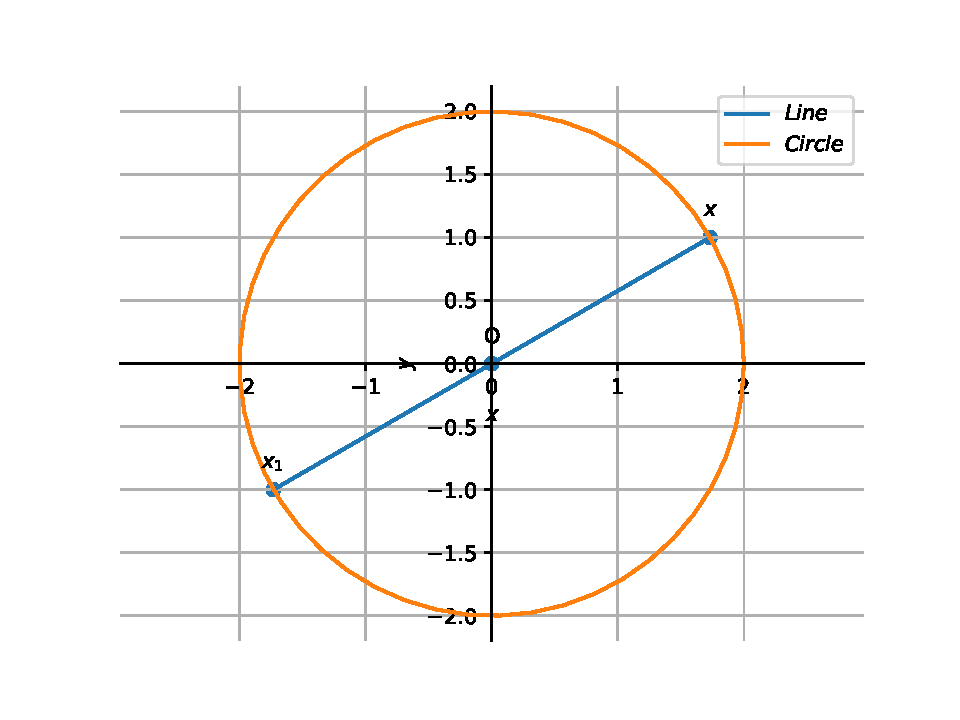
\includegraphics[width=0.75\columnwidth]{chapters/12/8/1/6/figs/conics-fig.pdf} 
		\caption{}
		\label{fig:12/8/1/6}
  	\end{figure}
  From the given information, the parameters of the  circle and line are
                      \begin{align}
			      f= -4, \vec{u}=\vec{0}, \vec{V}=\vec{I}, \vec{m}=\myvec{1 \\ \sqrt{3}}, \vec{h} = \vec{0}
		\label{eq:12/8/1/6}
                    \end{align}                                                                              
Substituting		    the above parameters in  
\eqref{eq:tangent_roots},
	  \begin{align}                                                                               
		  \mu= \sqrt{3}
	  \end{align}
	  yielding  
the desired point of intersection as                                               
\begin{align}
	\vec{x} = \myvec{\sqrt{3} \\ 1}                               
\end{align}
Note that we have chosen only the point of intersection in the first quadrant as shown in 
		\figref{fig:12/8/1/6}.
From
		\eqref{eq:12/8/1/6},
		the angle between the given line and the x axis is
\begin{align}
	\theta=30\degree
\end{align} 
and
the area of the sector is 
\begin{align}
	{\frac{\theta}{360}}\pi r^2=
	\frac{\pi}{3}
\end{align}

\item 
\label{chapters/12/8/1/7}
	\begin{figure}[H]
		\centering
 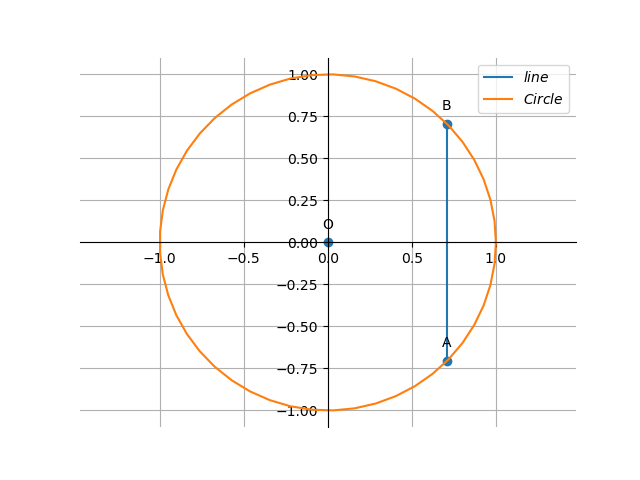
\includegraphics[width=0.75\columnwidth]{chapters/12/8/1/7/figs/conic.png}
		\caption{}
		\label{fig:12/8/1/7}
  	\end{figure}
The given circle can be expressed as a conic with parameters
\begin{align}
\vec{V}=
\myvec{
1 & 0\\
0 & 1
},
\vec{u}=0,
f=-a^2
\end{align} 
The given line 
parameters are
\begin{align} 
	\vec{h}=\myvec{\frac{a}{\sqrt{2}} \\ 0},  \vec{m}=\vec{e}_2.
\end{align}
Substituting the above in
\eqref{eq:tangent_roots},
\begin{align}
    \kappa =\pm\frac{a}{\sqrt{2}}
\end{align}
yielding the
points of intersection of the line with circle as
\begin{align}
    \vec{A}=\myvec{
\frac{a}{\sqrt{2}}\\
-\frac{a}{\sqrt{2}}
    },
    \vec{B}=\myvec{
\frac{a}{\sqrt{2}}\\
\frac{a}{\sqrt{2}}
    }
\end{align}
 From 
		\figref{fig:12/8/1/7},
the total area of the portion is given by
\begin{align}
	ar( APQ)&=2 ar (APR)
	\\
&=2\int_{0}^{\frac{a}{\sqrt{2}}}\sqrt{a^2-x^2}\,dx 
	\\
	&=\frac{a^2}{2}\brak{1+\frac{\pi}{2}}
\end{align}

\item 
\label{chapters/12/8/1/8}
\iffalse
\documentclass[journal,10pt,twocolumn]{article}
\usepackage{graphicx}
\usepackage[margin=0.5in]{geometry}
\usepackage[cmex10]{amsmath}
\usepackage{array}
\usepackage{booktabs}
\usepackage{mathtools}
\title{\textbf{Conic section Assignment}}
\author{Somisetty Kedareswari}
\date{October 2022}


\providecommand{\norm}[1]{\left\lVert#1\right\rVert}
\providecommand{\abs}[1]{\left\vert#1\right\vert}
\let\vec\mathbf
\newcommand{\myvec}[1]{\ensuremath{\begin{pmatrix}#1\end{pmatrix}}}
\newcommand{\mydet}[1]{\ensuremath{\begin{vmatrix}#1\end{vmatrix}}}
\providecommand{\brak}[1]{\ensuremath{\left(#1\right)}}
\providecommand{\lbrak}[1]{\ensuremath{\left(#1\right.}}
\providecommand{\rbrak}[1]{\ensuremath{\left.#1\right)}}
\providecommand{\sbrak}[1]{\ensuremath{{}\left[#1\right]}}

\begin{document}

\maketitle
\paragraph{\textit{Problem Statement} -
\fi

The area between $x = y^2$ and $x = 4$ is divided into two equal parts by the line $x = a$, find the value of a.
\\
\solution
	\begin{figure}[!h]
		\centering
 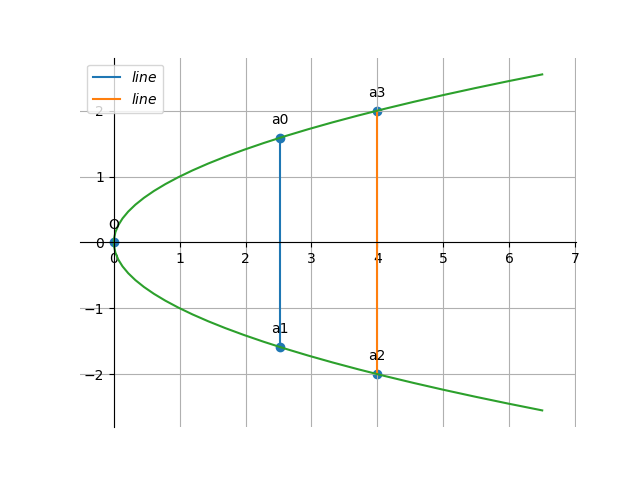
\includegraphics[width=\columnwidth]{chapters/12/8/1/8/figs/conics1.png}
		\caption{}
		\label{fig:12/8/1/8}
  	\end{figure}
	\iffalse
\section*{\large Solution}

\begin{figure}[h]
\centering
\includegraphics[width=1\columnwidth]{conics1.png}

\caption{The parabola formed by the curve $y^2 = x$ and the line x=4}
\label{fig:parabola}
\end{figure}

The given equation of parabola $y^2 = x$ can be written in the general quadratic form as
\begin{align}
    \label{eq:conic_quad_form}
    \vec{x}^{\top}\vec{V}\vec{x}+2\vec{u}^{\top}\vec{x}+f=0
    \end{align}
where
\fi
The given conic parameters are
\begin{align}
 \vec{V} = \myvec{0 & 0\\0 & 1},
	\vec{u} = -\frac{1}{2}\vec{e}_1
 f = 0
\end{align}
\iffalse


The point of intersection of the lines x=a and x=4 to the parabola is given by



The points of intersection of the line 
\begin{align}
 L: \quad \vec{x} = \vec{q} + \mu \vec{m} \quad \mu \in \mathbf{R}
\label{eq:conic_tangent}
\end{align}
with the conic section are given by
\begin{align}
\vec{x}_i = \vec{q} + \mu_i \vec{m}
\label{eq:conic_tangent_pts}
\end{align}
%
where
{\tiny
\begin{multline}
\mu_i = \frac{1}
{
\vec{m}^T\vec{V}\vec{m}
}
\lbrak{-\vec{m}^T\brak{\vec{V}\vec{q}+\vec{u}}}
\\
\pm
\rbrak{\sqrt{
\sbrak{
\vec{m}^T\brak{\vec{V}\vec{q}+\vec{u}}
}^2
-
\brak
{
\vec{q}^T\vec{V}\vec{q} + 2\vec{u}^T\vec{q} +f
}
\brak{\vec{m}^T\vec{V}\vec{m}}
}
}
\label{eq:tangent_roots}
\end{multline}
}
\fi

The parameters of the lines are
\begin{align}
\vec{q}_2=\myvec{a\\0},
\vec{m}_2=\vec{e}_2
\end{align}
Substituting the above values in 
\eqref{eq:tangent_roots},
\begin{align}
\mu_i=a,-a
\end{align}
yielding  the points of  intersection as
\begin{align}
\vec{a_0}=\myvec{a\\a},
\vec{a_1}=\myvec{a\\-a}
\end{align}
Similarly, for the line $x-4=0$, 
\begin{align}
\vec{q_1}=\myvec{4\\0},
\vec{m_1}=\vec{e}_2
\end{align}
yielding
\begin{align}
\mu_i=2,-2
\end{align}
and
\begin{align}
\vec{a}_3=\myvec{4\\2},
\vec{a}_2=\myvec{4\\-2}.
\end{align}
Area between parabola and the line $x=4$ is divided equally by the line $x=a$.  Thus, 
\begin{align}
	A_1&=\int_{0}^{a} \ \sqrt{x} \,dx
	\\
	A_2&=\int_{a}^{4} \ \sqrt{x} \,dx
	\\
	\text{ and }
	A_1&=A_2 \\
\implies 
	a&=4^\frac{2}{3}
\end{align}

\iffalse
\section*{\large Construction}

{
\setlength\extrarowheight{5pt}
\begin{tabular}{|l|c|}
    \hline 
    \textbf{Points} & \textbf{intersection points} \\ \hline
   a0 & $\myvec{
   a\\
   a
   } $ \\\hline
   a1 & $\myvec{
   a\\
   -a
   } $ \\\hline
    
   a3 & $\myvec{
   4\\
   2
   } $ \\\hline
   a2 & $\myvec{
   4\\
   -2
   } $ \\\hline
      
      \end{tabular}
}

\end{document}
\fi

\item 
\label{chapters/12/8/1/9}
\iffalse
\documentclass[10pt,a4paper]{report}
%\usepackage[latin1]{inputenc}
\usepackage[utf8]{inputenc}
\usepackage{amsmath}
\usepackage{amsfonts}
\usepackage{amssymb}
\usepackage{graphicx}
\usepackage{multicol}
\usepackage{tabularx}
\usepackage{tikz}
\usetikzlibrary{arrows,shapes,automata,petri,positioning,calc}
\usepackage{hyperref}
\usepackage{tikz}
\usetikzlibrary{matrix,calc}
\usepackage[margin=0.5in]{geometry}
% ---- power functions -----% 
\newcommand{\myvec}[1]{\ensuremath{\begin{pmatrix}#1\end{pmatrix}}}
\let\vec\mathbf

\providecommand{\norm}[1]{\left\lVert#1\right\rVert}
\providecommand{\abs}[1]{\left\vert#1\right\vert}
\let\vec\mathbf

\newcommand{\mydet}[1]{\ensuremath{\begin{vmatrix}#1\end{vmatrix}}}
\providecommand{\brak}[1]{\ensuremath{\left(#1\right)}}
\providecommand{\lbrak}[1]{\ensuremath{\left(#1\right.}}
\providecommand{\rbrak}[1]{\ensuremath{\left.#1\right)}}
\providecommand{\sbrak}[1]{\ensuremath{{}\left[#1\right]}}
%-------end power functions----%
\newenvironment{Figure}
  {\par\medskip\noindent\minipage{\linewidth}}
  {\endminipage\par\medskip}
\begin{document}
%--------------------logo figure-------------------------%
\begin{figure*}[!tbp]
  \centering
  \begin{minipage}[b]{0.4\textwidth}
    
\includegraphics[scale = 0.5]{iitlogo.png}
  \end{minipage}
  \vspace{0.2cm}
\end{figure*}
%--------------------name & rollno-----------------------
\raggedright \textbf{Name}:\hspace{1mm} Ganga Gopinath\hspace{3cm} \Large \textbf{Assignment-6}\hspace{2.5cm} % 
\normalsize \textbf{Roll No.} :\hspace{1mm} FWC22050\vspace{1cm}
\begin{multicols}{2}

%----------------problem statement--------------%
\raggedright \textbf{Problem Statement:}\vspace{2mm}
\raggedright \\ 
\fi
	Find the area of the region bounded by the parabola $y=x^2$ and $y= \abs{x}$.
	\\
	\solution
	\begin{figure}[!h]
		\centering
 \includegraphics[width=\columnwidth]{chapters/12/8/1/9/figs/con3.pdf}
		\caption{}
		\label{fig:12/8/1/9}
  	\end{figure}
	\iffalse
\vspace{5mm}
%-----------------------------solution---------------------------
\raggedright \textbf{SOLUTION}:\vspace{2mm}\\

%---------given----------------%
\raggedright \textbf{Given}:\vspace{2mm}\\

Equation of Parabola is \\ \vspace{1mm}
\begin{align}
x^2=4y 
\end{align}
Equation of line is \\\vspace{1mm}
\begin{align}
y=|x|
\end{align}
From (1) we can say that Parabola is symmetric about the positive y axis.\\ \vspace{2mm}
%-------------To find ------------------%
\textbf{To Find }\vspace{2mm}\\
To find the intersection points and area of shaded region shown in figure\vspace{2mm}  \\ 
%--------------steps----------------------%
\textbf{STEP-1}\vspace{2mm}\\
The given parabola and line can be expressed as conics with parameters,\\ \vspace{1mm}

For Parabola,\\\vspace{1mm}
The conic parameters are
\begin{align}
\vec{V}_1=\myvec{
1 & 0\\
0 & 0
}
\end{align} 

\begin{align}
\vec{u_1}= -\myvec{
0\\
\frac{1}{2}
}\
\end{align} 
\begin{align}
f_1=0
\end{align} \vspace{2mm}

For line,\\\vspace{1mm}
\begin{align}
\vec{V}_2=\myvec{
0 & 0\\
0 & 0
}
\end{align} 


\begin{align}
\vec{u_2}= \myvec{
-\frac{1}{2}\\
\frac{1}{2}
}\
\end{align} 
\begin{align}
f_2=0
\end{align} \vspace{2mm}


\textbf{STEP-2}\vspace{2mm}\\
The points of intersection of the line is given by, \\ 
\begin{align}
L: \quad \vec{x} = \vec{q} + \kappa \vec{m} \quad \kappa \in \mathbb{R}
\end{align}
with the conic section, \\ 
\begin{align}
	\vec{x}^{\top}\vec{V}\vec{x} + 2\vec{u}^{\top} \vec{x} + f = 0
\end{align}
are given by \\
\begin{align}
\vec{x}_i = \vec{q} + \kappa_i \vec{m}
\end{align}
where, \\
{\tiny
\begin{multline}
\kappa_i = \frac{1}
{
\vec{m}^T\vec{V}\vec{m}
}
\lbrak{-\vec{m}^T\brak{\vec{V}\vec{q}+\vec{u}}}
\\
\pm
\rbrak{\sqrt{
\sbrak{
\vec{m}^T\brak{\vec{V}\vec{q}+\vec{u}}
}^2
-
\brak
{
\vec{q}^T\vec{V}\vec{q} + 2\vec{u}^T\vec{q} +f
}
\brak{\vec{m}^T\vec{V}\vec{m}}
}
}
\end{multline}
}
On substituting\\
\begin{align}
\vec{q} &= \myvec{
0\\
0.25
} 
\end{align}
\begin{align}
\vec{m} = \myvec{1 \\ 0}
\end{align}
With the given Parabola,\\ 
\begin{align}
	\vec{V} &= \myvec{
1 & 0\\
0 & 0
    }
\end{align}
\begin{align}
	\vec{u} = -\myvec{\frac{1}{2} \\0}
 \end{align}
 \begin{align}
  f = 0
 \end{align}
The value of $\kappa$ ,\\
\begin{align}
    \kappa = 1,-1
\end{align}
The points of intersection with Parabola along circle are \\
\begin{align}
    \vec{A}=\myvec{
1\\
1
    }
\end{align}
\begin{align}
    \vec{B}=\myvec{
-1\\
1
    }
\end{align}
\textbf{Result}
\begin{center}
 \includegraphics[width=0.5\textwidth]{con3.pdf}  
 \end{center}\vspace{1mm}
 From the figure,\\ \vspace{1mm}
Total area of portion is given by, \\ \vspace{1mm}
\begin{align}
 A=  \int_{0}^{1} g(x)-f(x) \,dx 
\end{align}
Where g(x) is area under line and f(x) is the area of parabola \\ \vspace{1mm}
\begin{align}
A= \int_{0}^{1} y dx -\int_{0}^{1} y_1 dx  \\
A= \int_{0}^{1} x dx -\int_{0}^{1} x^2 dx  \\
\end{align}
Area A is,\\ 
\begin{align}
    A= .333\,m^2
\end{align}
 \vspace{2mm} \textbf{Construction}
\begin{center}
\setlength{\arrayrulewidth}{0.5mm}
\setlength{\tabcolsep}{6pt}
\renewcommand{\arraystretch}{1.5}
    \begin{tabular}{|l|c|}
    \hline 
    \textbf{Points} & \textbf{coordinates} \\ \hline
   $\vec{A}$ & $\myvec{
   1\\
   1
   } $ \\ \hline
   $\vec{B}$ & $\myvec{
   -1\\
   1
   } $ \\\hline
      \end{tabular}
  \end{center}

\raggedright  Download the code \\
https://github.com/Gangagopinath/ASSIGNMENT/tree/
\newline
main/assignment6
  \end{multicols}
\end{document}
Footer
\fi

\item 
\label{chapters/12/8/1/10}
\iffalse
\documentclass[10pt,a4paper]{report}
\usepackage[latin1]{inputenc}
\usepackage{amsmath}
\usepackage{amsfonts}
\usepackage{amssymb}
\usepackage{graphicx}
\usepackage{hyperref}
\usepackage{multicol}
\usepackage[margin=0.5in]{geometry}
\usepackage{tikz}
\usepackage[document]{ragged2e}
\usepackage{romannum}
\usetikzlibrary{arrows,shapes.gates.logic.US,shapes.gates.logic.IEC,calc}
\usepackage{titlesec}
\titlespacing{\subsection}{1pt}{\parskip}{3pt}
\titlespacing{\subsubsection}{0pt}{\parskip}{-\parskip}
\titlespacing{\paragraph}{0pt}{\parskip}{\parskip}
\newcommand{\myvec}[1]{\ensuremath{\begin{pmatrix}#1\end{pmatrix}}}
\let\vec\mathbf

\newcommand{\mydet}[1]{\ensuremath{\begin{vmatrix}#1\end{vmatrix}}}
\providecommand{\brak}[1]{\ensuremath{\left(#1\right)}}
\providecommand{\lbrak}[1]{\ensuremath{\left(#1\right.}}
\providecommand{\rbrak}[1]{\ensuremath{\left.#1\right)}}
\providecommand{\sbrak}[1]{\ensuremath{{}\left[#1\right]}}

\begin{document}

\begin{multicols}{2}
\raggedright {
\includegraphics[scale=0.06]{IITH logo.jpg}} \vspace{3mm}\\ \raggedleft Name:SHAIK KHAJA MASTAN AHMED\vspace{2mm}\\ 
\raggedleft Roll No.: FWC22052\vspace{2mm}\\ 
\raggedleft 19pa1a04e9@vishnu.edu.in \vspace{2mm}\\ 
\raggedleft Oct 2022 \vspace{5mm}\\
\end{multicols}

\centering \Large \textbf{MATRIX : CONIC ASSIGNMENT} \normalsize \vspace{10mm}

\begin{multicols}{2}

\section{Problem:}  
\fi
Find the area bounded by the curve $x^2=4y$ and the line $x=4y-2$.
\\
\solution 
	\begin{figure}[!h]
		\centering
 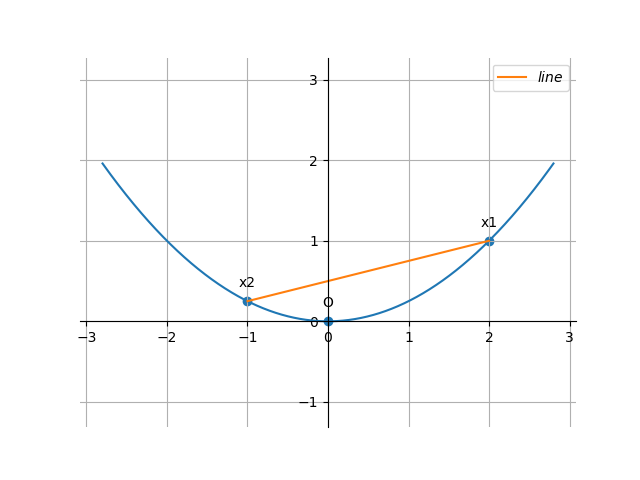
\includegraphics[width=\columnwidth]{chapters/12/8/1/10/figs/conic.png}
		\caption{}
		\label{fig:12/8/1/10}
  	\end{figure}
\iffalse

\section{Solution: }
\raggedright \textbf{Input Parameters :}\\ \vspace{2mm}
\centering Curve Equation : $x^2=4y$. \\ \vspace{1mm}
Line Equation : $x=4y-2$.\\
\vspace{3mm}

\raggedright \textbf{To Find :}\\ \vspace{2mm}
\begin{enumerate}
\item Comparing the given curve equation with the standard equation of the conics and finding it's parameters.
\item Finding the required parameters for the line equation.
\item Finding the Point of Intersection of the to the curve.
\item Finding the area bounded by the curve and the line.
\end{enumerate}

\raggedright \textbf{Step - 1 :}\\ \vspace{2mm}
Curve Equation : $x^2=4y$. \\ \vspace{1mm}
The standard equation of the conics is given as :
\begin{align}
\vec{x}^{\top}\vec{V}\vec{x}+2\vec{u}^{\top}\vec{x}+f=0
\end{align}
\fi
The given curve  can be expressed as a conic with parameters
\begin{align}
	\vec{V} &= \myvec{1 & 0\\0 & 0}, \vec{u} = \myvec{0 \\-2}, f = 0
	\end{align}
\iffalse

\raggedright \textbf{Step - 2 :}\\ \vspace{2mm}
Line Equation : $x=4y-2$. \\ \vspace{1mm}
\fi
The parameters of the given line are
\begin{align}
\vec{q} = \myvec{-2 \\0} , \vec{m}=\myvec{4\\1}
\end{align}
The points of intersection can then be obtained from \eqref{eq:tangent_roots} as
\iffalse

\raggedright \textbf{Step - 3 :}\\ \vspace{2mm}
The points of intersection of the line, \\ 
\begin{align}
L: \quad \vec{x} = \vec{q} + \mu \vec{m} \quad \mu \in \mathbb{R}
\end{align}
with the conic section, \\ 
\begin{align}
	\vec{x}^{\top}\vec{V}\vec{x} + 2\vec{u}^{\top} \vec{x} + f = 0
\end{align}
are given by \\
\begin{align}
\vec{x}_i = \vec{q} + \mu_i \vec{m}
\end{align}
where, \\
{\tiny
\begin{multline}
\mu_i = \frac{1}
{
\vec{m}^T\vec{V}\vec{m}
}
\lbrak{-\vec{m}^T\brak{\vec{V}\vec{q}+\vec{u}}}
\\
\pm
\rbrak{\sqrt{
\sbrak{
\vec{m}^T\brak{\vec{V}\vec{q}+\vec{u}}
}^2
-
\brak
{
\vec{q}^T\vec{V}\vec{q} + 2\vec{u}^T\vec{q} +f
}
\brak{\vec{m}^T\vec{V}\vec{m}}
}
}
\end{multline}
}
\raggedright On substituting $\vec{V},\vec{q} ,\vec{m}$ in the above equation,
we get the values of $\mu$. By substituting the values of $\mu$ in eq(6), \\we get the points of intersection of line with the given curve. \\
\centering $i.e., \vec{x}_1,\vec{x}_2$\\ 
\fi

\begin{align}
\therefore \vec{x}_1=\myvec{2\\1} , \vec{x}_2=\myvec{-1\\ \frac{1}{4}}
\end{align}
\iffalse

\raggedright \textbf{Step - 4 :}\\ \vspace{2mm}
The area bounded by the curve $x^2=4y$ and line $x=4y-2$ is given by\\
\fi
The desired area is then obtained as
\begin{align}
	A&=\int_{x_2}^{x_1} [f(x)-g(x)] \,dx
	\\
	&=\int_{-1}^{2} \brak{\frac{x+2}{4}-\frac{x^2}{4}} \,dx
	\\
	& = \frac{9}{8} 
\end{align}
\iffalse

\raggedright \textbf{Code Link :}\\ \vspace{2mm}
The below link realises the code of the above construction.\\
\begin{center}
\fbox{\parbox{8.5cm}{\url{https://github.com/19pa1a04e9/FWC-IITH/tree/main/Assignment-1/MATRICES/Conic/codes/conic.py}}}
\end{center}


\section{Termux Commands :}
\centering bash rncom.sh ..... Using Shell commands.


\section{Plot :} 
\begin{center}
  \includegraphics[scale=0.55]{conic.png}
  Figure 1
  	\end{center}

 
\end{multicols}
\end{document}
\fi

\item Find the area of the region bounded by the curve ${y}^2
= 4{x}$ and the line ${x} = 3$.
\label{chapters/12/8/1/11}
\end{enumerate}
Choose the correct answer in the following   Exercises 12 and 13.
\begin{enumerate} [resume]
\item Area lying in the first quadrant and bounded by the circle ${x}^2 + {y}^2 = 4$ and the lines ${x} = 0$ and ${x} = 2$ is \break
\label{chapters/12/8/1/12}
\begin{enumerate}[itemsep=+2mm]
\item $\pi$
\item $\dfrac{\pi}{2}$
\item $\dfrac{\pi}{3}$  
\item $\dfrac{\pi}{4}$
\end{enumerate}
\item Find the area of the region bounded by the curve $y^2 = 4x$, y-axis and the line $y = 3$. 
\label{chapters/12/8/1/13}
\\
\solution
In this case, 
\begin{align}
	\vec{V} &= \myvec{ 0 & 0 \\ 0 & 1} \\
	\vec{u} &= \myvec{-2 \\ 0} \\
	f &= 0
\end{align}
For the given line $y=3$, the parameters are
\begin{align}
	\vec{h} = \myvec{0 \\ 3} , \vec{m} = \myvec{1 \\ 0 }
\end{align}
The intersection of 
the line with the conic is obtained from \eqref{eq:tangent_roots} 
as
\begin{align}
	\kappa  = \frac{9}{4} 
\end{align}
The point of contact is given as
\begin{align}
	\vec{a}_0 = \myvec{\frac{9}{4}  \\[1pt] \\ 3}
\end{align}
From \figref{fig:chapters/12/8/1/13/Fig1},
the desired area of the region is obtaioned as
\begin{align}
	\int_{0}^{3} \ \frac{y^2}{4} \,dy &= \frac{1}{12}\sbrak{y^3}_{0}^{3} \\
	&= \frac{1}{12}\brak{27-0} \\
	&= \frac{9}{4} \text{ sq.units}
\end{align}
\begin{figure}[!h]
	\begin{center}
		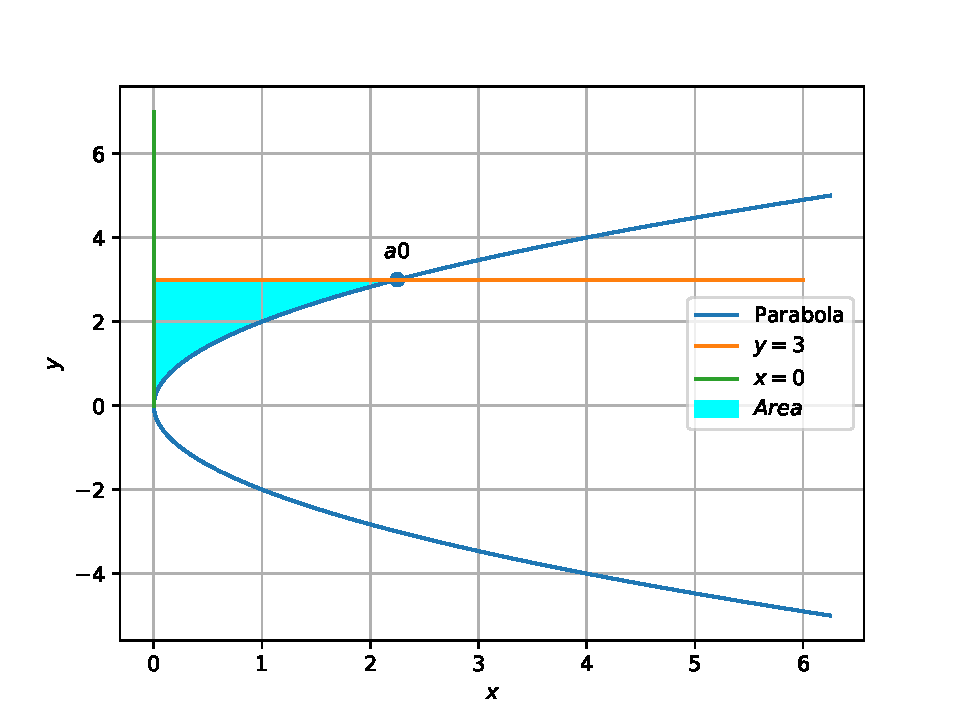
\includegraphics[width=\columnwidth]{chapters/12/8/1/13/figs/problem13.pdf}
	\end{center}
\caption{}
\label{fig:chapters/12/8/1/13/Fig1}
\end{figure}

\item 
\label{chapters/12/8/3/3}
	\begin{figure}[H]
		\centering
 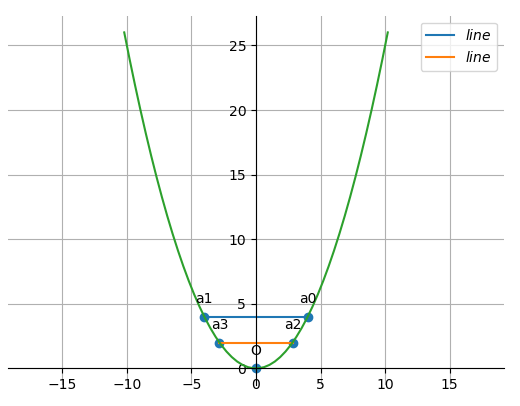
\includegraphics[width=0.75\columnwidth]{chapters/12/8/3/3/figs/conic.png}
		\caption{}
		\label{fig:12/8/3/3}
  	\end{figure}
The conic parameters are
\begin{align}
	\vec{V} = \myvec{1 & 0\\0 & 0},
	\vec{u} = \myvec{0\\-2},
	f = 0
	%\\
\end{align}
The vector parameters of 
$y-4=0$
are
\begin{align}
	\vec{h}_1=\myvec{0\\4},
	\vec{m}_1=\myvec{1\\0}
\end{align}
Substituting the above in \eqref{eq:tangent_roots},
\begin{align}
\kappa_i=4,-4
\end{align}
yielding
the points of intersection with the parabola as
\begin{align}
\vec{a}_0=\myvec{4\\4},
\vec{a}_1=\myvec{-4\\4}
\end{align}
Similarly, for 
the line $y-2=0$, the vector parameters are
\begin{align}
\vec{h}_2=\myvec{0\\2},
\vec{m}_2=\myvec{1\\0}
\end{align}
yielding 
\begin{align}
\kappa_i=2.8,-2.8
\end{align}
and the points of intersection
\begin{align}
\vec{a}_2=\myvec{2.8\\2},
\vec{a}_3=\myvec{-2.8\\2}
\end{align}
From 
		\figref{fig:12/8/3/3},
the area of the parabola between the lines $y=2$ and $y=4$ is given by
\begin{align}
\int_{0}^{4} \ 2\sqrt{y} \,dy-\int_{0}^{2} \ 2\sqrt{y} \,dy
=6.895 
\end{align}

\item 
\label{chapters/12/8/3/7}
\iffalse
\documentclass[10pt,a4paper]{report}
%\usepackage[latin1]{inputenc}
\usepackage[utf8]{inputenc}
\usepackage{amsmath}
\usepackage{amsfonts}
\usepackage{amssymb}
\usepackage{graphicx}
\usepackage{multicol}
\usepackage{tabularx}
\usepackage{tikz}
\usetikzlibrary{arrows,shapes,automata,petri,positioning,calc}
\usepackage{hyperref}
\usepackage{tikz}
\usetikzlibrary{matrix,calc}
\usepackage[margin=0.5in]{geometry}
% ---- power functions -----% 
\newcommand{\myvec}[1]{\ensuremath{\begin{pmatrix}#1\end{pmatrix}}}
\let\vec\mathbf

\providecommand{\norm}[1]{\left\lVert#1\right\rVert}
\providecommand{\abs}[1]{\left\vert#1\right\vert}
\let\vec\mathbf

\newcommand{\mydet}[1]{\ensuremath{\begin{vmatrix}#1\end{vmatrix}}}
\providecommand{\brak}[1]{\ensuremath{\left(#1\right)}}
\providecommand{\lbrak}[1]{\ensuremath{\left(#1\right.}}
\providecommand{\rbrak}[1]{\ensuremath{\left.#1\right)}}
\providecommand{\sbrak}[1]{\ensuremath{{}\left[#1\right]}}
%-------end power functions----%
\newenvironment{Figure}
  {\par\medskip\noindent\minipage{\linewidth}}
  {\endminipage\par\medskip}
\begin{document}
%--------------------logo figure-------------------------%
\begin{figure*}[!tbp]
  \centering
  \begin{minipage}[b]{0.4\textwidth}
    
\includegraphics[scale=0.05]{iitlogo.jpg} 
  \end{minipage}
  \hfill
  \vspace{5mm}\begin{minipage}[b]{0.4\textwidth}
\raggedleft  
\includegraphics[scale=0.05]{nrc.png}  \

  \end{minipage}\vspace{0.2cm}
\end{figure*}
%--------------------name & rollno-----------------------
\raggedright \textbf{Name}:\hspace{1mm} Cheenepalli Chandana\hspace{2cm} \Large \textbf{Conic Assignment}\hspace{2.5cm} % 
\normalsize \textbf{Roll No.} :\hspace{1mm} FWC22062\vspace{1cm}
\begin{multicols}{2}

%----------------problem statement--------------%
\raggedright \textbf{Problem Statement:}\vspace{2mm}
\raggedright \\
\fi
	Find the area enclosed by the parabola $4y=3x^2 $ and the line $2y=3x+12$.\\
	\solution
	\begin{figure}[!h]
		\centering
 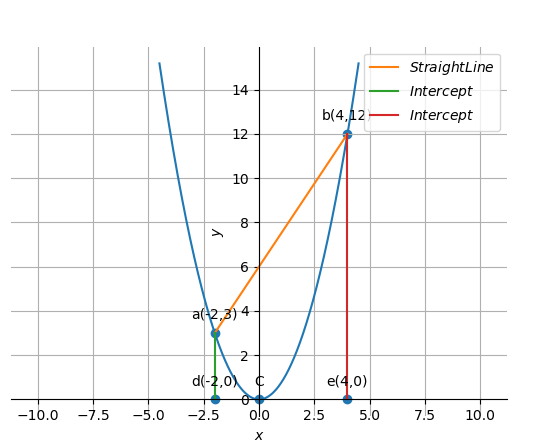
\includegraphics[width=\columnwidth]{chapters/12/8/3/7/figs/conic.png}
		\caption{}
		\label{fig:12/8/3/7}
  	\end{figure}
\iffalse
\vspace{5mm}
%-----------------------------solution---------------------------
\raggedright \textbf{SOLUTION}:\vspace{2mm}\\

%---------given----------------%
\raggedright \textbf{Given}:\vspace{2mm}\\
Equation of parabola is \\\vspace{1mm}
\begin{align}
4y=3x^2
\end{align}
Equation of line is \\ \vspace{1mm}
\begin{align}
2y=3x+12
\end{align}
%-------------To find ------------------%
\textbf{To Find }\vspace{2mm}\\
To find the intersection points and area enclosed by the parabola and line shown in figure\vspace{2mm}  \\ 
%--------------steps----------------------%
\textbf{STEP-1}\vspace{2mm}\\
The given parabola can be expressed as conics with parameters,\\ \vspace{1mm}
\begin{align}
	\vec{x}^{\top}\vec{V}\vec{x} + 2\vec{u}^{\top} \vec{x} + f = 0
\end{align}
\fi
The parameters of the given conic are
\begin{align}
\vec{V}=\myvec{
3 & 0\\
0 & 0
},
\vec{u}=\myvec{0\\-2},
f=0.
\end{align} 
For the line, the parameters are
\iffalse
\textbf{STEP-2}\vspace{2mm}\\
the given line equation can be written as\\ 
\begin{align} 
	\vec{n}^{\top}\vec{X}=c
\end{align}
Where
\begin{align}
\vec{n}=\myvec{-3\\2},\vec{m}=\myvec{2\\3}
\end{align}
\textbf{STEP-3}\vspace{2mm}\\
The points of intersection of the line, \\ 
\begin{align}
L: \quad \vec{x} = \vec{q} + \kappa \vec{m} \quad \kappa \in \mathbb{R}
\end{align}
with the conic section, \\ 
\begin{align}
	\vec{x}^{\top}\vec{V}\vec{x} + 2\vec{u}^{\top} \vec{x} + f = 0
\end{align}
are given by \\
\begin{align}
\vec{x}_i = \vec{q} + \kappa_i \vec{m}
\end{align}
where, \\
{\tiny
\begin{multline}
\kappa_i = \frac{1}
{
\vec{m}^T\vec{V}\vec{m}
}
\lbrak{-\vec{m}^T\brak{\vec{V}\vec{q}+\vec{u}}}
\\
\pm
\rbrak{\sqrt{
\sbrak{
\vec{m}^T\brak{\vec{V}\vec{q}+\vec{u}}
}^2
-
\brak
{
\vec{q}^T\vec{V}\vec{q} + 2\vec{u}^T\vec{q} +f
}
\brak{\vec{m}^T\vec{V}\vec{m}}
}
}
\end{multline}
}
On substituting\\
\fi
\begin{align}
\vec{h} = \myvec{
-2\\
3
},
\vec{m} = \myvec{2 \\ 3}
\end{align}
\iffalse
With the given parabola as in eq(3),(4),(5),\\ 

The value of $\kappa$ ,\\
\fi
yielding
\begin{align}
    \mu=-2.5,2.7
\end{align}
upon substitution in \eqref{eq:tangent_roots}
resulting in the points of intersection
\iffalse
by substituting eq(13) in eq(6)we get the
points of intersection of line with parabola \\
\fi
\begin{align}
    \vec{A}=\myvec{
-2\\
3
    },
    \vec{B}=\myvec{
4\\
12
    }.
\end{align}
From Fig. 
		\ref{fig:12/8/3/7},
		\iffalse
\textbf{Result}
\begin{center}
 \includegraphics[scale=0.5]{conic.png}    
 \end{center}\vspace{1mm}
 From the figure,\\ \vspace{1mm}
Total area of portion is given by, \\ \vspace{1mm}
Total Area=(area enclosed by the line)-(area of parabola under the line )

\subsection*{Area Under the line}
\fi
the desired area is 
\begin{align}
\int_{-2}^{4} \frac{3x+12}{2} \,dx
-\int_{-2}^{4}\frac{3x^2}{4} \,dx 
= 27 
\end{align}
\iffalse
 \vspace{2mm} \textbf{Construction}
\begin{center}
\setlength{\arrayrulewidth}{0.5mm}
\setlength{\tabcolsep}{6pt}
\renewcommand{\arraystretch}{1.5}
    \begin{tabular}{|l|c|}
    \hline 
    \textbf{Points} & \textbf{coordinates} \\ \hline
   B & $\myvec{
   4\\
   12
   } $ \\\hline
   A & $\myvec{
   -2\\
   3
   } $ \\\hline
      \end{tabular}
  \end{center}
  \end{multicols}
 
Get the python code of the figures from

\begin{table}[h]
\large
\centering
\framebox{
\url{https://github.com/chandana531/cchandana_fwc/blob/main/conic_assignment/code/conic.py}}
\bibliographystyle{ieeetr}
\end{table} 
 
\end{document}
 
\fi

\item 
\label{chapters/12/8/3/8}
	\begin{figure}[!h]
		\centering
 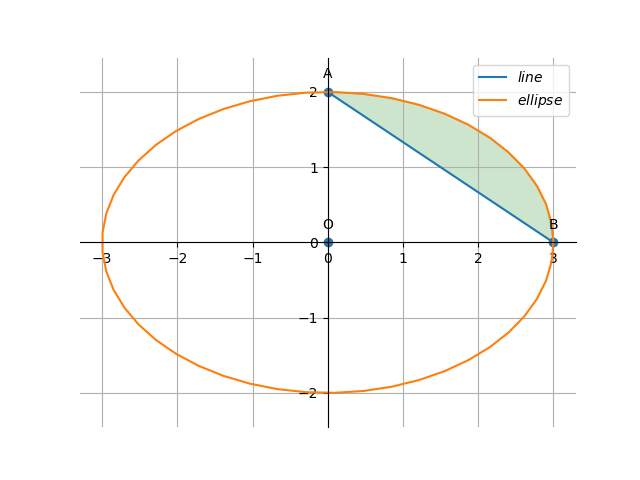
\includegraphics[width=\columnwidth]{chapters/12/8/3/8/figs/conic_fig.png}
		\caption{}
		\label{fig:12/8/3/8}
  	\end{figure}
The given ellipse can be expressed as conics with parameters
\begin{align}
\vec{V}=\myvec{
b^2 & 0\\
0 & a^2
},
\vec{u}=0,
f=-(a^2b^2).
\end{align} 
The line parameters are
\begin{align}
\vec{h} &= \myvec{
a\\
0
},
\vec{m} = \myvec{\frac{1}{b} \\ -\frac{1}{a}}.
\end{align}
Substituting the given parameters in \eqref{eq:tangent_roots},
\begin{align}
    \mu=0,-6
\end{align}
yielding the points of intersection
\begin{align}
    \vec{A}=\myvec{
a\\
0
    },
    \vec{B}=\myvec{
0\\
b
    }.
\end{align}
From 
		\figref{fig:12/8/3/8},
the desired area is
\begin{multline}
\int_{0}^{a}\frac{b}{a}\sqrt{a^2-x^2} \,dx 
-\int_{0}^{a} \frac{b}{a}(a-x) \,dx
\\
	= \frac{ab}{2}\brak{\frac{\pi}{2}-1}
	= 3\brak{\frac{\pi}{2}-1}
\end{multline}
upon substituting $a=3, b=2$.

\item 
\label{chapters/12/8/3/9}
\iffalse
\documentclass[10pt,a4paper]{report}
%\usepackage[latin1]{inputenc}
\usepackage[utf8]{inputenc}
\usepackage{amsmath}
\usepackage{amsfonts}
\usepackage{amssymb}
\usepackage{graphicx}
\usepackage{multicol}
\usepackage{tabularx}
\usepackage{tikz}
\usetikzlibrary{arrows,shapes,automata,petri,positioning,calc}
\usepackage{hyperref}
\usepackage{tikz}
\usetikzlibrary{matrix,calc}
\usepackage[margin=0.5in]{geometry}
% ---- power functions -----% 
\newcommand{\myvec}[1]{\ensuremath{\begin{pmatrix}#1\end{pmatrix}}}
\let\vec\mathbf

\providecommand{\norm}[1]{\left\lVert#1\right\rVert}
\providecommand{\abs}[1]{\left\vert#1\right\vert}
\let\vec\mathbf

\newcommand{\mydet}[1]{\ensuremath{\begin{vmatrix}#1\end{vmatrix}}}
\providecommand{\brak}[1]{\ensuremath{\left(#1\right)}}
\providecommand{\lbrak}[1]{\ensuremath{\left(#1\right.}}
\providecommand{\rbrak}[1]{\ensuremath{\left.#1\right)}}
\providecommand{\sbrak}[1]{\ensuremath{{}\left[#1\right]}}
%-------end power functions----%
\newenvironment{Figure}
  {\par\medskip\noindent\minipage{\linewidth}}
  {\endminipage\par\medskip}
\begin{document}
%--------------------logo figure-------------------------%
\begin{figure*}[!tbp]
  \centering
  \begin{minipage}[b]{0.4\textwidth}
    
\includegraphics[scale=0.05]{fig/iitlogo.jpg} 
  \end{minipage}
  \hfill
  \vspace{5mm}\begin{minipage}[b]{0.4\textwidth}
\raggedleft  
\includegraphics[scale=0.05]{fig/nrc.png}  \

  \end{minipage}\vspace{0.2cm}
\end{figure*}
%--------------------name & rollno-----------------------
\raggedright \textbf{Name}:\hspace{1mm} kanekal kousar\hspace{3cm} \Large \textbf{Conic Assignment}\hspace{2.5cm} % 
\normalsize \textbf{Roll No.} :\hspace{1mm} FWC22063\vspace{1cm}
\begin{multicols}{2}

%----------------problem statement--------------%
\raggedright \textbf{Problem Statement:}\vspace{2mm}
\raggedright \\
\fi
	Find the area of the smaller region bounded by the ellipse $\frac{x^2}{a^2}+\frac{y^2}{b^2}=1$
and the line $\frac{x}{a}+\frac{y}{b}=1$.\\
\solution
	\begin{figure}[!h]
		\centering
 \includegraphics[width=\columnwidth]{chapters/12/8/3/9/figs/conic_fig.png}    
		\caption{}
		\label{fig:12/8/3/9}
  	\end{figure}
\iffalse
\vspace{5mm}
%-----------------------------solution---------------------------
\raggedright \textbf{SOLUTION}:\vspace{2mm}\\

%---------given----------------%
\raggedright \textbf{Given}:\vspace{2mm}\\
Equation of ellipse is \\\vspace{1mm}
\begin{align}
\frac{x^2}{a^2}+\frac{y^2}{b^2}=1
\end{align}
Equation of line is \\ \vspace{1mm}
\begin{align}
\frac{x}{a}+\frac{y}{b}=1
\end{align}
%-------------To find ------------------%
\textbf{To Find }\vspace{2mm}\\
To find the intersection points and area of shaded region shown in figure\vspace{2mm}  \\ 
%--------------steps----------------------%
\textbf{STEP-1}\vspace{2mm}\\
\fi
The given ellipse can be expressed as a conic with parameters
\begin{align}
\vec{V}=\myvec{
b^2 & 0\\
0 & a^2
},
\vec{u}=0,
f=-(a^2b^2).
\end{align}
\iffalse
\textbf{STEP-2}\vspace{2mm}\\
\fi
The given line parameters are
\iffalse
\begin{align} 
	\vec{x}=\begin{pmatrix}a \\ 0 \\ \end{pmatrix}+k\begin{pmatrix}\frac{1}{b} \\ -\frac{1}{a} \\ \end{pmatrix}
\end{align}

\textbf{STEP-3}\vspace{2mm}\\
The points of intersection of the line, \\ 
\begin{align}
L: \quad \vec{x} = \vec{q} + \kappa \vec{m} \quad \kappa \in \mathbb{R}
\end{align}
with the conic section, \\ 
\begin{align}
	\vec{x}^{\top}\vec{V}\vec{x} + 2\vec{u}^{\top} \vec{x} + f = 0
\end{align}
are given by \\
\begin{align}
\vec{x}_i = \vec{q} + \kappa_i \vec{m}
\end{align}
where, \\
{\tiny
\begin{multline}
\kappa_i = \frac{1}
{
\vec{m}^T\vec{V}\vec{m}
}
\lbrak{-\vec{m}^T\brak{\vec{V}\vec{q}+\vec{u}}}
\\
\pm
\rbrak{\sqrt{
\sbrak{
\vec{m}^T\brak{\vec{V}\vec{q}+\vec{u}}
}^2
-
\brak
{
\vec{q}^T\vec{V}\vec{q} + 2\vec{u}^T\vec{q} +f
}
\brak{\vec{m}^T\vec{V}\vec{m}}
}
}
\end{multline}
}
On substituting\\
\fi
\begin{align}
\vec{h} &= \myvec{
a\\
0
}, 
\vec{m} = \myvec{\frac{1}{b} \\ -\frac{1}{a}}.
\end{align}
Substituting the given parameters in \eqref{eq:tangent_roots}
\iffalse
With the given ellipse as in eq(3),(4),(5),\\ 

The value of $\kappa$ ,\\
\fi
\begin{align}
    \mu=0,-6
\end{align}
yielding
\iffalse
by substituting eq(13) in eq(6)we get the
\fi
the points of intersection 
\begin{align}
    \vec{A}=\myvec{
a\\
0
    },
    \vec{B}=\myvec{
0\\
b
    }
\end{align}
From Fig.
		\ref{fig:12/8/3/9},
		\iffalse
\textbf{Result}
\begin{center}
 \includegraphics[scale=0.5]{fig/conic_fig.png}    
 \end{center}\vspace{1mm}
 From the figure,\\ \vspace{1mm}
Total area of portion is given by, \\ \vspace{1mm}
Total Area=(area of ellipse in first quadrant)-(area of a triangle\textbf{AOB})

\subsection*{Area of triangle}

\fi
the desired area is
\begin{align}
\int_{0}^{a}\frac{b}{a}\sqrt{a^2-x^2} \,dx 
-\int_{0}^{a} \frac{b}{a}(a-x) \,dx
	= \frac{ab}{2}\brak{\frac{\pi}{2}-1}
\end{align}
\iffalse
 \vspace{2mm} \textbf{Construction}
\begin{center}
\setlength{\arrayrulewidth}{0.5mm}
\setlength{\tabcolsep}{6pt}
\renewcommand{\arraystretch}{1.5}
    \begin{tabular}{|l|c|}
    \hline 
    \textbf{Points} & \textbf{coordinates} \\ \hline
   B & $\myvec{
   a\\
   0
   } $ \\\hline
   A & $\myvec{
   0\\
   b
   } $ \\\hline
      \end{tabular}
  \end{center}
  \end{multicols}
 
Get the python code of the figures from

\begin{table}[h]
\large
\centering
\framebox{
\url{https://github.com/kkousar/KOUSAR_FWC/blob/main/conics/code/conic.py}}
\bibliographystyle{ieeetr}
\end{table} 
 
\end{document}
 
\fi

\item 
\label{chapters/12/8/3/10}
\iffalse
\documentclass[journal,10pt,twocolumn]{article}
\usepackage{graphicx}
\usepackage[margin=0.5in]{geometry}
\usepackage[cmex10]{amsmath}
\usepackage{array}
\usepackage{booktabs}
\usepackage{mathtools}
\title{\textbf{Conic section Assignment}}
\author{P.Revathi}
\date{October 2022}


\providecommand{\norm}[1]{\left\lVert#1\right\rVert}
\providecommand{\abs}[1]{\left\vert#1\right\vert}
\let\vec\mathbf
\newcommand{\myvec}[1]{\ensuremath{\begin{pmatrix}#1\end{pmatrix}}}
\newcommand{\mydet}[1]{\ensuremath{\begin{vmatrix}#1\end{vmatrix}}}
\providecommand{\brak}[1]{\ensuremath{\left(#1\right)}}
\providecommand{\lbrak}[1]{\ensuremath{\left(#1\right.}}
\providecommand{\rbrak}[1]{\ensuremath{\left.#1\right)}}
\providecommand{\sbrak}[1]{\ensuremath{{}\left[#1\right]}}

\begin{document}

\maketitle
\paragraph{\textit{Problem Statement} -
\fi
Find the area of the region bounded by the curve $x^2=y$ and the lines $y=x+2$ and the $x$ axis.
\\
\solution 
	\begin{figure}[!h]
		\centering
 \includegraphics[width=\columnwidth]{chapters/12/8/3/10/figs/conics1.png}
		\caption{}
		\label{fig:12/8/3/10}
  	\end{figure}
\iffalse

\section*{\large Solution}

\begin{figure}[h]
\centering
\includegraphics[width=1\columnwidth]{conics1.png}

%\caption{The parabola formed by the curve $y^2 = 9x$ and the lines x=2 and x=4}
\label{fig:parabola}
\end{figure}

The given equation of parabola $x^2 = y$ can be written in the general quadratic form as
\begin{align}
    \label{eq:conic_quad_form}
    \vec{x}^{\top}\vec{V}\vec{x}+2\vec{u}^{\top}\vec{x}+f=0
    \end{align}
where
The parameters of the given conic are
\begin{align}
 \vec{V} = \myvec{1 & 0\\0 & 0},
 \vec{u} = \myvec{0\\-0.5},
 f = 0
\end{align}
The points of intersection of the line 
\begin{align}
 L: \quad \vec{x} = \vec{q} + \mu \vec{m} \quad \mu \in \mathbf{R}
\label{eq:conic_tangent}
\end{align}
with the conic section are given by
\begin{align}
\vec{x}_i = \vec{q} + \mu_i \vec{m}
\label{eq:conic_tangent_pts}
\end{align}
%
where
{\tiny
\begin{multline}
\mu_i = \frac{1}
{
\vec{m}^T\vec{V}\vec{m}
}
\lbrak{-\vec{m}^T\brak{\vec{V}\vec{q}+\vec{u}}}
\\
\pm
\rbrak{\sqrt{
\sbrak{
\vec{m}^T\brak{\vec{V}\vec{q}+\vec{u}}
}^2
-
\brak
{
\vec{q}^T\vec{V}\vec{q} + 2\vec{u}^T\vec{q} +f
}
\brak{\vec{m}^T\vec{V}\vec{m}}
}
}
\label{eq:tangent_roots}
\end{multline}
}
The parameters of the line $y=x+2$ are
\begin{align}
\vec{h}=\myvec{0\\2},
\vec{m}=\myvec{1\\1}
\end{align}
yielding
\begin{align}
\mu_i=-2
\end{align}
upon substituting in \eqref{eq:tangent_roots}.     The points of intersection of this line with the conic are
\begin{align}
\vec{a_0}=\myvec{2\\4},
\vec{a_1}=\myvec{-1\\1}
\end{align}
Similarly, 
Given line equation y=x+2\\

$$x-y=-2$$\\
$$\vec{n}^{t}\vec{x}=c$$\\
$$\vec{x}=\vec{A}+\lambda \vec{m}$$\\
%\end{centre}


$$\vec{x}=\begin{pmatrix}
-2\\ 
0
\end{pmatrix}+\mu \begin{pmatrix}
1\\ 
1
\end{pmatrix}$$\\

Substitute the x value in the quadratic equation then we get a quadratic equations
\begin{align}
    \label{eq:conic_quad_form}
    \vec{x}^{\top}\vec{V}\vec{x}+2\vec{u}^{\top}\vec{x}+f=0
    \end{align}
    
$$\mu ^{2}-3\mu +2=0\\$$
$$\mu =1,2\\$$
$$\mu ^{2}-\mu\\$$
$$\mu =1,0\\$$
The resultant x values are\\
$$\vec{x}=\begin{pmatrix}
-2\\ 
0
\end{pmatrix}$$\\
$$\vec{x}=\begin{pmatrix}
-1\\ 
1
\end{pmatrix}$$\\
$$\vec{x}=\begin{pmatrix}
0\\ 
2
\end{pmatrix}$$

Area of the parabola in between the lines parabola and y=x+2 is given by
\begin{align}
\implies A_1=\int_{-2}^{-1} \ x+2 \,dx
\end{align}

\begin{align}
\implies A_2=\int_{-1}^{0} \ x^2 \,dx
\end{align}
\begin{align}
\implies A_1+A_1=\int_{-2}^{-1} \ x+2 \,dx+\int_{-1}^{0} \ x^2 \,dx
\end{align}
\begin{align}
\implies A_1+ A_2=\frac{5}{6}sq units
\end{align}

\end{document}
\fi

\item 
\label{chapters/12/8/3/17}
\iffalse
\def\mytitle{MATRICES USING PYTHON(CONIC)}
\def\myauthor{R.Radhika}
\def\contact{r170234@rguktrkv.ac.in}
\def\mymodule{Future Wireless Communication (FWC)}
\documentclass[10pt, a4paper]{article}
\usepackage[a4paper,outer=1.5cm,inner=1.5cm,top=1.75cm,bottom=1.5cm]{geometry}
\twocolumn
\usepackage{graphicx}
\graphicspath{{./images/}}
\usepackage[colorlinks,linkcolor={black},citecolor={blue!80!black},urlcolor={blue!80!black}]{hyperref}
\usepackage[parfill]{parskip}
\usepackage{lmodern}
\usepackage{tikz}
	\usepackage{physics}
%\documentclass[tikz, border=2mm]{standalone}
%\usepackage{karnaugh-map}
%\documentclass{article}
\usepackage{tabularx}
%\usepackage{circuitikz}
\usepackage{enumitem}
\usetikzlibrary{calc}
\usepackage{amsmath}
\usepackage{amssymb}
\renewcommand*\familydefault{\sfdefault}
\usepackage{watermark}
\usepackage{lipsum}
\usepackage{xcolor}
\usepackage{listings}
\usepackage{float}
\usepackage{titlesec}
\providecommand{\mtx}[1]{\mathbf{#1}}
\titlespacing{\subsection}{1pt}{\parskip}{3pt}
\titlespacing{\subsubsection}{0pt}{\parskip}{-\parskip}
\titlespacing{\paragraph}{0pt}{\parskip}{\parskip}
\newcommand{\figuremacro}[5]{
    \begin{figure}[#1]
        \centering
        \includegraphics[width=#5\columnwidth]{#2}
        \caption[#3]{\textbf{#3}#4}
        \label{fig:#2}
    \end{figure}
}

\newcommand{\myvec}[1]{\ensuremath{\begin{pmatrix}#1\end{pmatrix}}}
\let\vec\mathbf
\lstset{
frame=single, 
breaklines=true,
columns=fullflexible
}

\title{\mytitle}
\author{\myauthor\hspace{1em}\\\contact\\FWC22066\hspace{6.5em}IITH\hspace{0.5em}\mymodule\hspace{6em}Assignment}
\begin{document}
	\maketitle
	\tableofcontents
   \section{Problem}
   \fi
Find   the area bounded by the curve $y=x|x|, x$-axis and the ordinates $x$=-1 and $x$=1.
\\
\solution 
	\begin{figure}[!h]
		\centering
 \includegraphics[width=\columnwidth]{chapters/12/8/3/17/figs/conicfig.pdf}
		\caption{}
		\label{fig:12/8/3/17}
  	\end{figure}
   \iffalse
[Hint: y=$x^2$ if $x>0$  and y=$-x^2$ if $x<0$]
   					
\section{Construction}
  \includegraphics[scale=0.47]{conicfig.pdf}
  	\begin{center}
  Figure of construction
  	\end{center}
  \section{Solution}
  
\raggedright\large{ Draw the ordinates by using $x$=1 and $x$=-1. Then we need to draw  two parabolas using  given hint [Hint: y=$x^2$ if $x>0$  and y=$-x^2$ if $x<0$]for that we need to find out the area bounded by the curve  y=$x|x|$  .}
\vspace{2mm}\\
\raggedright\large{Then the limits from -1 to 1  and the points(-1,-1),(1,1)}\vspace{2mm}\\
The standard conic equation\\
\begin{align}
\vec{x}^{\top}\vec{V}\vec{x}+2\vec{u}^{\top}\vec{x}+f=0
\end{align}
\begin{align}
\vec{x}^{\top}\vec{V}\vec{x}+2\vec{u_1}^{\top}\vec{x}+f_1=0
\end{align}
\fi
The parameters of the given conics are
\begin{align}
	\vec{V}_1&=\myvec{1&0\\0&0} ,\vec{u_1}=\myvec{0\\-\frac{1}{2}},  f_1=0
	\\
	\vec{V}_2&=\myvec{-1&0\\0&0} ,\vec{u_2}=\myvec{0\\-\frac{1}{2}},  f_2=0
\end{align}
The determinant equation for the intersection of two conics is 
\iffalse
\begin{align}
|\myvec{\vec{V_1}+\mu{\vec{V_2}}&\vec{u_1}+\mu{\vec{u_2}}\\\vec{u_1}+\mu{\vec{u_2}}&0}|
\end{align}
substitute eq 3 and 4 in eq 6\\
\fi
\begin{align}
\mydet{1-\mu&0&0\\0&0&-\frac{1}{2}-\frac{\mu}{2}\\0&-\frac{1}{2}-\frac{\mu}{2}&0} = 0
\end{align}
yielding,
\begin{align}
	\mu^3+\mu^2-\mu-1&=0
	\\
	\implies
	\mu&=-1, 1, 1
\end{align}
\iffalse
\begin{align}
|\vec{V_1}+\mu\vec{V_2}|<0
\end{align}
substitute $\vec{V_1}$ and $\vec{V_2}$ in eq-9\\
we get 0\\
\begin{align}
\vec{x}=\vec{q}+\mu{\vec{m}}
\end{align}
\begin{align}
q=\vec{V^{-1}}(k\vec{n}-\vec{u})
\end{align}
\begin{align}
k=\pm\sqrt{\frac{\norm{\vec{u_2}}^2\vec{V}-f}{\vec{n}^{\top}\vec{V^{-1}}\vec{n}}}
\end{align}
$\vec{n}=\myvec{1\\-1}$\\
$\vec{m}=\myvec{1\\1}$\\

by solving eq 10 and 11 we get\\
\begin{align}
\vec{q}=\myvec{0\\0}
\end{align}


 Given equation :  y=$x|x|$\\

We know that \\
\begin{equation}
   |x| =
    \begin{cases}
      x, & {x\geq0}\\
      -x & {x<0}\\
    \end{cases}       
\end{equation}

	Therefore,
\begin{equation}
   y=x|x| =
    \begin{cases}
      xx, & {x\geq0}\\
      x(-x) & {x<0}\\
    \end{cases}       
\end{equation}
\begin{equation}
   y =
    \begin{cases}
      x^2, & {x\geq0}\\
      -x^2 & {x<0}\\
    \end{cases}       
\end{equation}
Area Required=Area ABO+Area DCO\\
\textbf{Area of DCO}

Area  : \[ \int_{-1}^{1} y \,dx \]

Here, y=$x|x|$

Therefore Area DCO: \[ \int_{-1}^{0} -x^2 \,dx \]

 yielding ,\\
 
   -1/3 \\
 
 $|(-1/3)|$=1/3\\
 
 Area of DCO= 1/3

\textbf{Area  of ABO}: \[ \int_{0}^{1} x^2 \,dx \]

    yielding 1/3\\
   
     
     Area of ABO= 1/3
     

\textbf{Required Area=ABO+DCO}:
  1/3+1/3=2/3
Below python code realizes the above construction 

\begin{table}[h!]
    \begin{tabular}{|c|}
    \hline
         https://github.com/Radhikarkv/fwcproject.git\\
	\hline
    \end{tabular}
\end{table}
\end{document}
\fi

\item 
\label{chapters/12/8/2/3}
\iffalse
\documentclass[journal,12pt,twocolumn]{IEEEtran}
\usepackage[none]{hyphenat}
\usepackage{graphicx}
\usepackage{listings}
\usepackage[english]{babel}
\usepackage{graphicx}
\usepackage{caption} 
\usepackage{amsmath}
\usepackage{hyperref}
\usepackage{amsmath,amsfonts,amssymb}
\usepackage{booktabs}
\usepackage{array}
\let\vec\mathbf

\title{\textbf{\\Conics Assignment}}
\author{Sinkona Chinthamalla - FWC22054}

\newcommand{\myvec}[1]{\ensuremath{\myvec{#1}}}
\newcommand{\mydet}[1]{\ensuremath{\begin{vmatrix}#1\end{vmatrix}}}
\providecommand{\brak}[1]{\ensuremath{\left(#1\right)}}
\providecommand{\lbrak}[1]{\ensuremath{\left(#1\right.}}
\providecommand{\rbrak}[1]{\ensuremath{\left.#1\right)}}
\providecommand{\sbrak}[1]{\ensuremath{{}\left[#1\right]}}

\begin{document}
\maketitle

\section{Question}
\textbf {
\fi
	Find the area of the region bounded by the curves $y=x^2+2$, $y=x$, $x=0$ and $x=3. $
	\\
	\solution 
	\begin{figure}[!h]
		\centering
 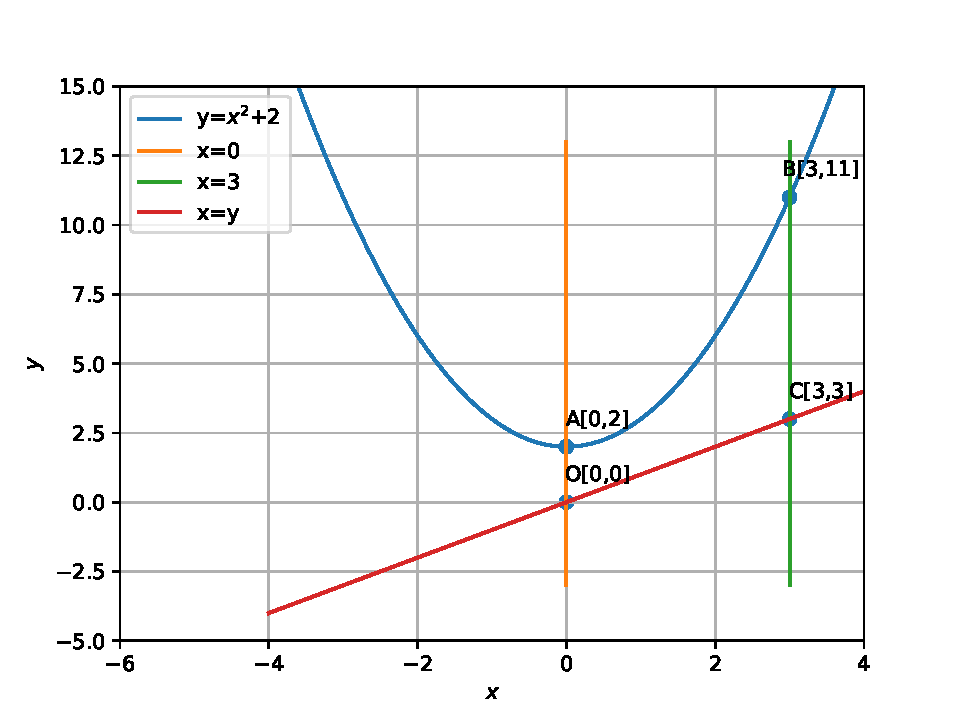
\includegraphics[width=\columnwidth]{chapters/12/8/2/3/figs/conic1.pdf}
		\caption{}
		\label{fig:12/8/2/3}
  	\end{figure}
	\iffalse

\begin{figure}[h!]
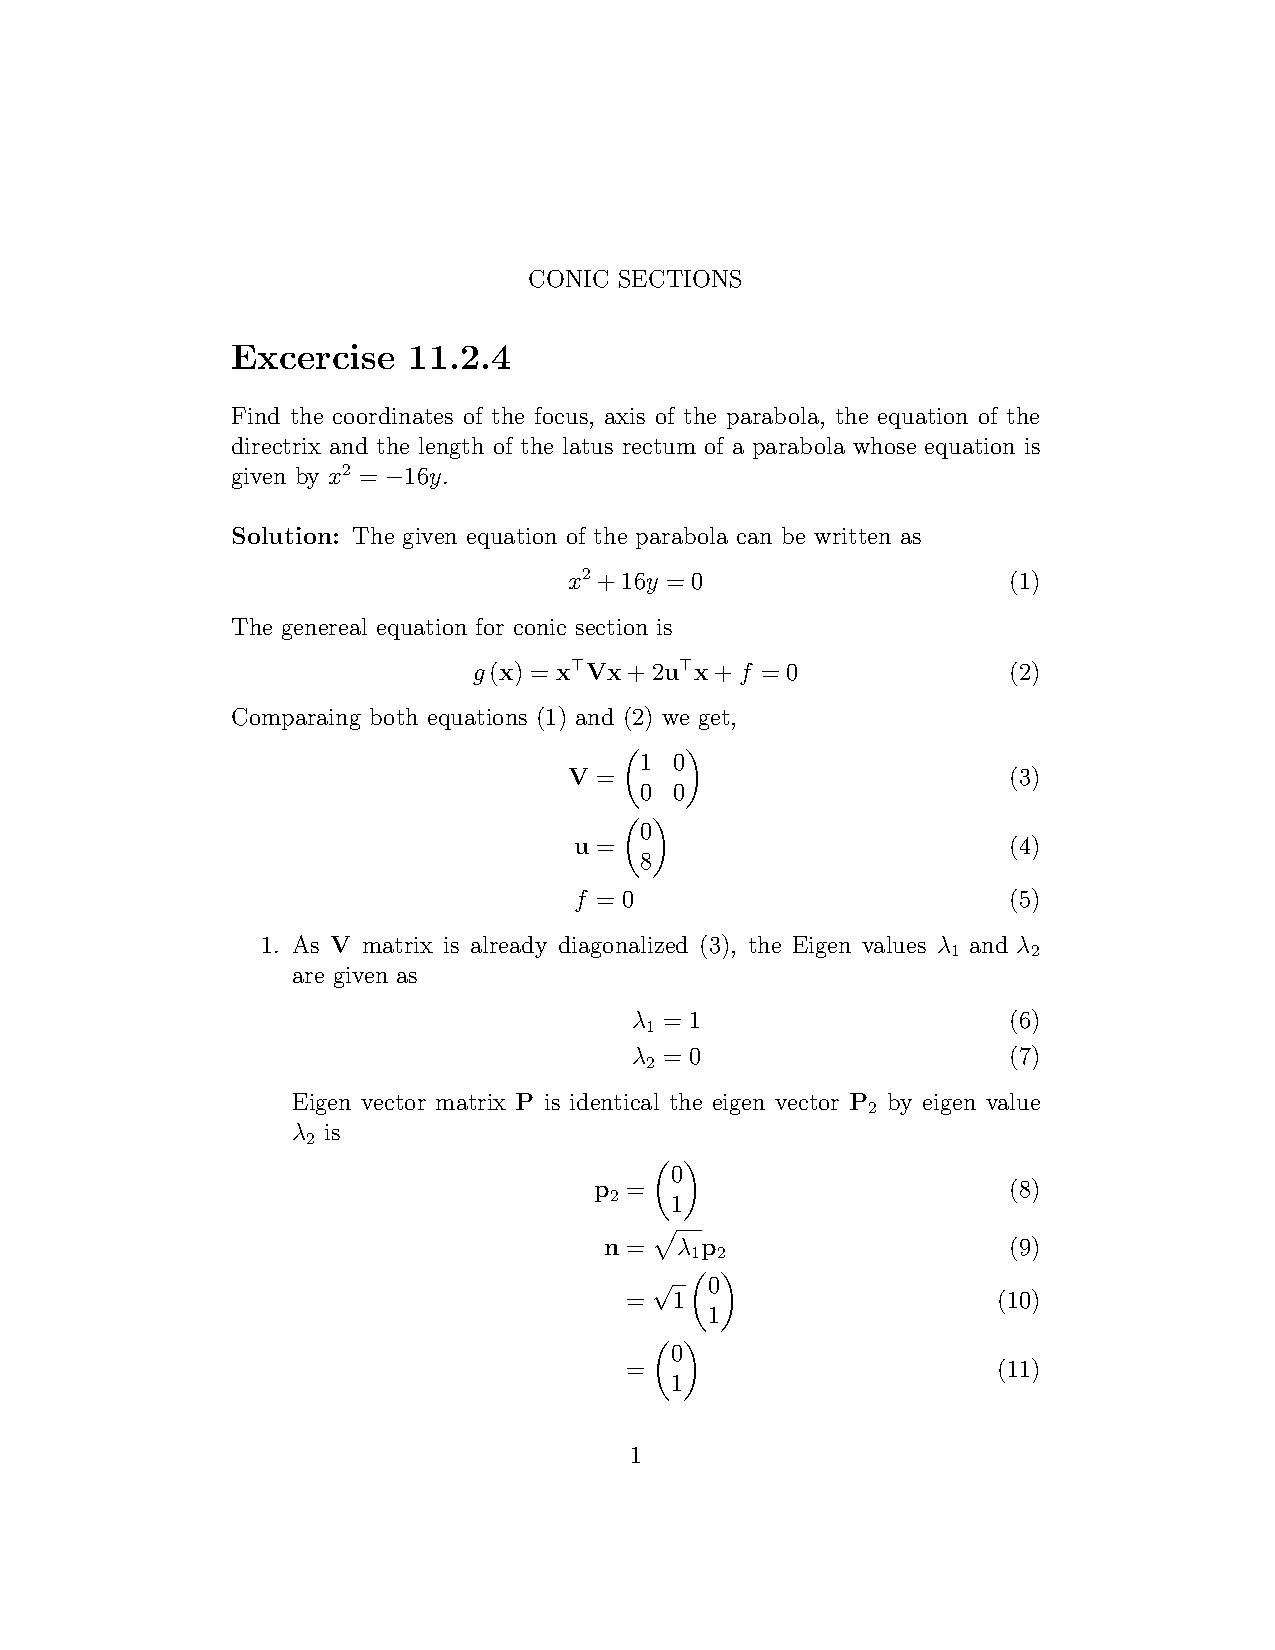
\includegraphics[scale=0.55]{conic1.pdf }
\end{figure}

\section{Construction}
\centering
\vspace{0.2cm}
{
\setlength\extrarowheight{2pt}
\begin{tabular}{|c|c|c|}
	\hline
	\textbf{Symbol}&\textbf{Value}&\textbf{Description}\\
	\hline
	\textbf{A} & 
	$ \myvec{
      0 \\
      2
    }$ & $\vec{q_1} $\\
	\hline
	B & 
	$\myvec{
     3 \\
     11
    }$ & $\vec{q_2} $\\
	\hline
	C & 
	$\myvec{
     3 \\
     3
    }$ & $\vec{q_3} $\\
	\hline
	O & 
	$\myvec{
     0 \\
     0
    }$ & $\vec{q_4} $\\
	\hline
\end{tabular}
}

\section{Solution}
\raggedright The equation of a conic with directrix $\vec{n}^\intercal\vec{x} = c$, eccentricity e and focus \textbf{F} is given by
\begin{align}
\vec{x}^{\top}\vec{V}\vec{x}+2\vec{u}^{\top}\vec{x}+f = 0 
\end{align}
where
\fi
The conic parameters are
\begin{align}
\vec{V} = \myvec{
1 & 0\\
0 & 0
}, 
\vec{u} = \myvec{
      0 \\
     -1/2
    },  
f = 2.  
\end{align}
\iffalse

\textbf{Finding Points of Intersection}
\vspace{0.2cm}
\\1. Consider line 
The intersection of the line
\begin{align}
%\myvec{
% 1 & 0
%} \vec{x} = 0 \\ 
\vec{x} = \mu\vec{e_2},
\end{align}
with the given conic is 
\begin{align}
\vec{q_1}^{\top}\vec{V}\vec{q_1}+2\vec{u}^{\top}\vec{q_1}+f = 0 \\
y_1^2\vec{e_2}^{\top}\vec{V}\vec{e_2}+2y_1\vec{u}^{\top}\vec{e_2}+f = 0 
\end{align}  
The value of $y_1$ is given by \\
\vspace{0.2cm}
1. when $\vec{e_2}^{\top}\vec{V}\vec{e_2} \neq 0 $ 
\begin{align}
y_1=\frac{-b_1 \pm \sqrt{b_1^2-4a_1c_1}}{2a_1} 
\end{align}
where,
\begin{align*}
a_1 & = \vec{e_2}^{\top}\vec{V}\vec{e_2}  \\
b_1 & = 2\vec{u}^{\top}\vec{e_2}  \\
c_1 & = f
\end{align*}

\vspace{0.2cm}
2. when $\vec{e_2}^{\top}\vec{V}\vec{e_2} = 0 $ 
\begin{align}
y_1=\frac{-f}{2\vec{u}^{\top}\vec{e_2}} 
\end{align} 

From (2) and $\vec{e_2}$, $\vec{e_2}^{\top}\vec{V}\vec{e_2} = 0 $ \\
Therefore, $y_1$ is obtained by substituting (3), (4) and $\vec{e_2}$ in (10).

\vspace{0.4cm}
2. Now consider line 
\begin{align}
\myvec{
 1 & 0
} \vec{x} = 3 \\
\vec{q_2} = y_2\vec{e_2}+3\vec{e_1}
\end{align}

To find the point of intersection of the Parabola with (11), substitute (12) in (1)
\begin{align}
\vec{q_2}^{\top}\vec{V}\vec{q_2}+2\vec{u}^{\top}\vec{q_2}+f = 0 
\end{align}
\begin{equation*}
y_2^2\vec{e_2}^{\top}\vec{V}\vec{e_2}+3y_2\vec{e_2}^{\top}\vec{V}\vec{e_1}+3y_2\vec{e_1}^{\top}\vec{V}\vec{e_2}+9\vec{e_1}^{\top}\vec{V}\vec{e_1}
\end{equation*}
\begin{equation}
+2y_2\vec{u}^{\top}\vec{e_2}+6\vec{u}^{\top}\vec{e_1}+f = 0 
\end{equation}

\vspace{0.2cm}
The value of $y_2$ is given by \\
\vspace{0.2cm}
1. when $\vec{e_2}^{\top}\vec{V}\vec{e_2} \neq 0 $ 
\begin{align}
y_2=\frac{-b_2 \pm \sqrt{b_2^2-4a_2c_2}}{2a_2} 
\end{align}
where,
\begin{align*}
a_2 & = \vec{e_2}^{\top}\vec{V}\vec{e_2}\\
b_2 & = 3\vec{e_2}^{\top}\vec{V}\vec{e_1}+3\vec{e_1}^{\top}\vec{V}\vec{e_2}+2\vec{u}^{\top}\vec{e_2} \\
c_2 & = 9\vec{e_1}^{\top}\vec{V}\vec{e_1}+6\vec{u}^{\top}\vec{e_1}+2 
\end{align*}

\vspace{0.2cm}
2. when $\vec{e_2}^{\top}\vec{V}\vec{e_2} = 0 $ 
\begin{align}
y_2=\frac{-f-9\vec{e_1}^{\top}\vec{V}\vec{e_1}}{2\vec{u}^{\top}\vec{e_2}} 
\end{align} 

From (2) and $\vec{e_2}$, $\vec{e_2}^{\top}\vec{V}\vec{e_2} = 0 $\\
Therefore, $d_2$ is obtained by substituting (2), (3), (4), $\vec{e_1}$ and $\vec{e_2}$ in (16). 

\vspace{0.4cm}
Therefore, the Points of Intersection of (5) and (11) with the given parabola are
\begin{align}
\vec{q_1} = \myvec{
 0\\
 2
} 
\end{align}
and 
\begin{align}
\vec{q_2} = \myvec{
 3\\
 11
} 
\end{align}
respectively.

\vspace{0.2cm}
The Points of Intersection of (11) and (5) with the line
\begin{align}
\myvec{
 1 & -1
} \vec{x} = 0
\end{align}  are
\begin{align}
\vec{q_3} = \myvec{
 3\\
 3
} 
\end{align}
\begin{align}
\vec{q_4} = \myvec{
 0\\
 0
} 
\end{align}
and

respectively.

\vspace{0.2cm}
\textbf{Finding area of the bounded region} \\
From Fig. 1, the area covered by the parabola is given by
\begin{align}
\int_{0}^{3} (x^2+2)dx =  \frac{x^3}{3} + 2x \Big|_0^3 \\
=15 
\end{align}

The area covered by (19) is given by
\begin{align}
\int_{0}^{3} xdx =  \frac{x^2}{2} \Big|_0^3 \\
= \frac{9}{2}
\end{align}

Thus, the desired area is the bounded region in
\\Fig. 1, and is given by
\begin{align}
\frac{21}{2} \quad sq.units
\end{align}

%\vspace{0.2cm}
%Get the python code from
%\begin{table}[h]
%\large
%\centering
%\begin{tabular}{|l|}
%\hline
%https://github.com/SinkonaChinthamalla/fwc/
%\\blob/main/matrix/conics/codes \\
%\hline
%\end{tabular}
%\end{table}	
\end{document}
\fi

\item 
\label{chapters/12/8/2/6}
\iffalse
\documentclass[journal,12pt,twocolumn]{IEEEtran}
\usepackage{graphicx}
\usepackage{listings}
\usepackage[utf8]{inputenc}
\usepackage{caption}
\usepackage{hyperref}
\usepackage[cmex10]{amsmath}
\usepackage{array}
\usepackage{gensymb}
\usepackage{booktabs}
\usepackage{etoolbox}
\usepackage{amssymb}
\patchcmd{\section}{\centering}{}{}{}
\providecommand{\norm}[1]{\left\lVert#1\right\rVert}
\providecommand{\abs}[1]{\left\vert#1\right\vert}
\let\vec\mathbf

\makeatletter
\newcommand\xleftrightarrow[2][]{%
  \ext@arrow 9999{\longleftrightarrowfill@}{#1}{#2}}
\newcommand\longleftrightarrowfill@{%
  \arrowfill@\leftarrow\relbar\rightarrow}
\makeatother
\title{Matrix Problems \textbf{\\Conics }}
\author{Manoj Chavva} 
\newcommand{\myvec}[1]{\ensuremath{\begin{pmatrix}#1\end{pmatrix}}}
\newcommand{\mydet}[1]{\ensuremath{\begin{vmatrix}#1\end{vmatrix}}}
\providecommand{\brak}[1]{\ensuremath{\left(#1\right)}}
\providecommand{\lbrak}[1]{\ensuremath{\left(#1\right.}}
\providecommand{\rbrak}[1]{\ensuremath{\left.#1\right)}}
\providecommand{\sbrak}[1]{\ensuremath{{}\left[#1\right]}}

\begin{document}
\maketitle
\section{Problem Statement}

\noindent 
\fi
Find the smaller area enclosed by the circle $x^2 + y^2 = 4$ and the line $x + y = 2$. 
\\
\solution
	\begin{figure}[!h]
		\centering
 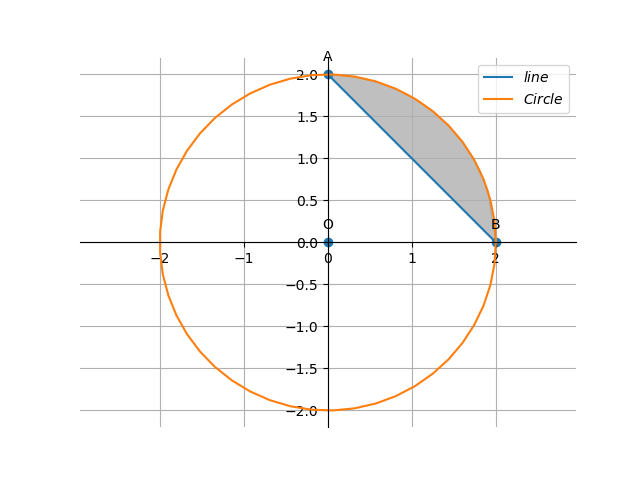
\includegraphics[width=\columnwidth]{chapters/12/8/2/6/figs/conic.png}
		\caption{}
		\label{fig:12/8/2/6}
  	\end{figure}
\iffalse
\begin{enumerate}
\item $2(\pi -2)$
\item $\pi -2$
\item $2\pi -1$
\item $2(\pi +2)$
\end{enumerate}


\begin{figure}[h]
\includegraphics[width=1\columnwidth]{./figs/conic.png}
\caption{Smaller region between Circle and Line}
\label{fig:conic}
\end{figure}

\raggedright \textbf{Given}: \\
Equation of circle is  
\begin{align} x^2 + y^2 = 4
\end{align}
Equation of line is 
\begin{align}
x+y=2
\end{align}
\textbf{To Find:} \\
To find the intersection points and area of shaded region shown in figure\
\section{Construction}

\begin{table}[h!]
\begin{center}
\setlength{\arrayrulewidth}{0.5mm}
\renewcommand{\arraystretch}{1.5}
    \begin{tabular}{|l|c|}
    \hline 
    \textbf{Points} & \textbf{coordinates} \\ \hline
   $\vec{A}$ & $\myvec{
   0\\
   2
   } $ \\\hline
   $\vec{B}$ & $\myvec{
   2\\
   0
   } $ \\\hline
      \end{tabular}
  \end{center}
\end{table}
\newpage
\section{solution}
\fi
The given circle can be expressed as conics with parameters,
\begin{align}
\vec{V}=\myvec{
4 & 0\\
0 & 4
},
\vec{u}=0,
f=-16
\end{align}
\iffalse

The given line equation can be written as\\ 
\begin{align} 
	\vec{x}=\begin{pmatrix}2 \\ 0 \\ \end{pmatrix}+k\begin{pmatrix}\frac{1}{2} \\ -\frac{1}{2} \\ \end{pmatrix}
\end{align}
The points of intersection of the line, \\ 
\begin{align}
L: \quad \vec{x} = \vec{q} + \kappa \vec{m} \quad \kappa \in \mathbb{R}
\end{align}

with the conic section, \\ 
\begin{align}
	\vec{x}^{\top}\vec{V}\vec{x} + 2\vec{u}^{\top} \vec{x} + f = 0
\end{align}
are given by \\
\begin{align}
\vec{x}_i = \vec{q} + \kappa_i \vec{m}
\end{align}
where, \\

\begin{equation*}
\kappa_i = \frac{1}
{
\vec{m}^T\vec{V}\vec{m}
}
\lbrak{-\vec{m}^T\brak{\vec{V}\vec{q}+\vec{u}}}
\pm
\end{equation*}
\begin{align}
\rbrak{\sqrt{
\sbrak{
\vec{m}^T\brak{\vec{V}\vec{q}+\vec{u}}
}^2
-
\brak
{
\vec{q}^T\vec{V}\vec{q} + 2\vec{u}^T\vec{q} +f
}
\brak{\vec{m}^T\vec{V}\vec{m}}
}
}
\end{align}
On substituting\\
\fi
The line parameters are
\begin{align}
\vec{h} &= \myvec{
2\\
0
}, 
\vec{m} = \myvec{\frac{1}{2} \\ -\frac{1}{2}}
\end{align}
\iffalse
With the given as in eq(3),(4),(5),\\ 

The value of $\kappa$ ,\\
\fi
Substituting the parameters in \eqref{eq:tangent_roots},
\begin{align}
\mu =0,-4
\end{align}
yielding the points of intersection as
   \iffalse 
By substituting eq(13) in eq(6) we get the
points of intersection of line with circle \\
\fi
\begin{align}
    \vec{A}=\myvec{
0\\
2
    },
    \vec{B}=\myvec{
2\\
0
    }
\end{align}
From Fig. 
		\ref{fig:12/8/2/6},
		\iffalse
Total area of portion is given by,\\ 
Total Area=(area of circle in first quadrant)-(area of a triangle \textbf{AOB})

\subsection*{Area of triangle}
\fi
the desired area is
\begin{align}
\int_{0}^{2}\sqrt{4-x^2} \,dx 
-\int_{0}^{2} (2-x) \,dx
=\pi - 2
\end{align}
\iffalse
By solving the above equation we get area of triangle as 2 units
\subsection*{Area of circle}

\begin{align} 
\implies A_2=\int_{0}^{2}\sqrt{4-x^2} \,dx 
\end{align}
By solving the above equation we get area of circle $\pi$

The total area is
$\implies \vec{A}=\pi - 2$


\begin{table}[h]
\large
\begin{tabular}{lll}
\multicolumn{3}{l}{Get Python Code for image from}                                                 \\ \hline
\multicolumn{3}{|l|}{\url{https://github.com/ManojChavva/FWC/blob/main/Matrix/conics/code/conic.py}} \\ 
 \hline
\multicolumn{3}{l}{Get LaTex code from}                                                            \\ \hline
\multicolumn{3}{|l|}{\url{https://github.com/ManojChavva/FWC/blob/main/Matrix/conics/conic.tex}}            \\ \hline
\end{tabular}
\end{table}



\end{document}




\fi

\end{enumerate}
